\chapter{文脈を考慮した一般単語感情推定手法}	

	\section{全体の概要}
	単語に対して想起される感情は,その単語が用いられる文脈に応じて変化するといえる.
	例えば「ドライブ」という単語について考えたとき,
	「海までドライブに行って気持ちよかった.」という文脈で用いられた場合には,
	喜などのポジティブな感情を想起すると考えられる.
	しかし,「ドライブで事故にあってしまった」という文脈で用いられた場合には,
	怖などのネガティブな感情を想起すると考えられる.
	このように,単語に対して想起される感情は文脈によって異なる.
	本手法では,単語から想起される感情を文脈によって変化させる.
	これにより,対話システムに応用するなど,後続のタスクで用いやすい形の
	感情情報を与えることが期待される.

	本手法では,BERTから得られる単語分散表現を活用することにより,
	同一単語に対しても文脈に応じて出力される感情ベクトルを変化させる.
	具体的には,BERTの出力する単語分散表現が文脈に応じて変化する性質を利用し,
	出力される感情ベクトルを変化させている.
	図\ref{fig:flowchart}は提案手法の流れを示したものである.
	\begin{figure}[H]
		\centering
		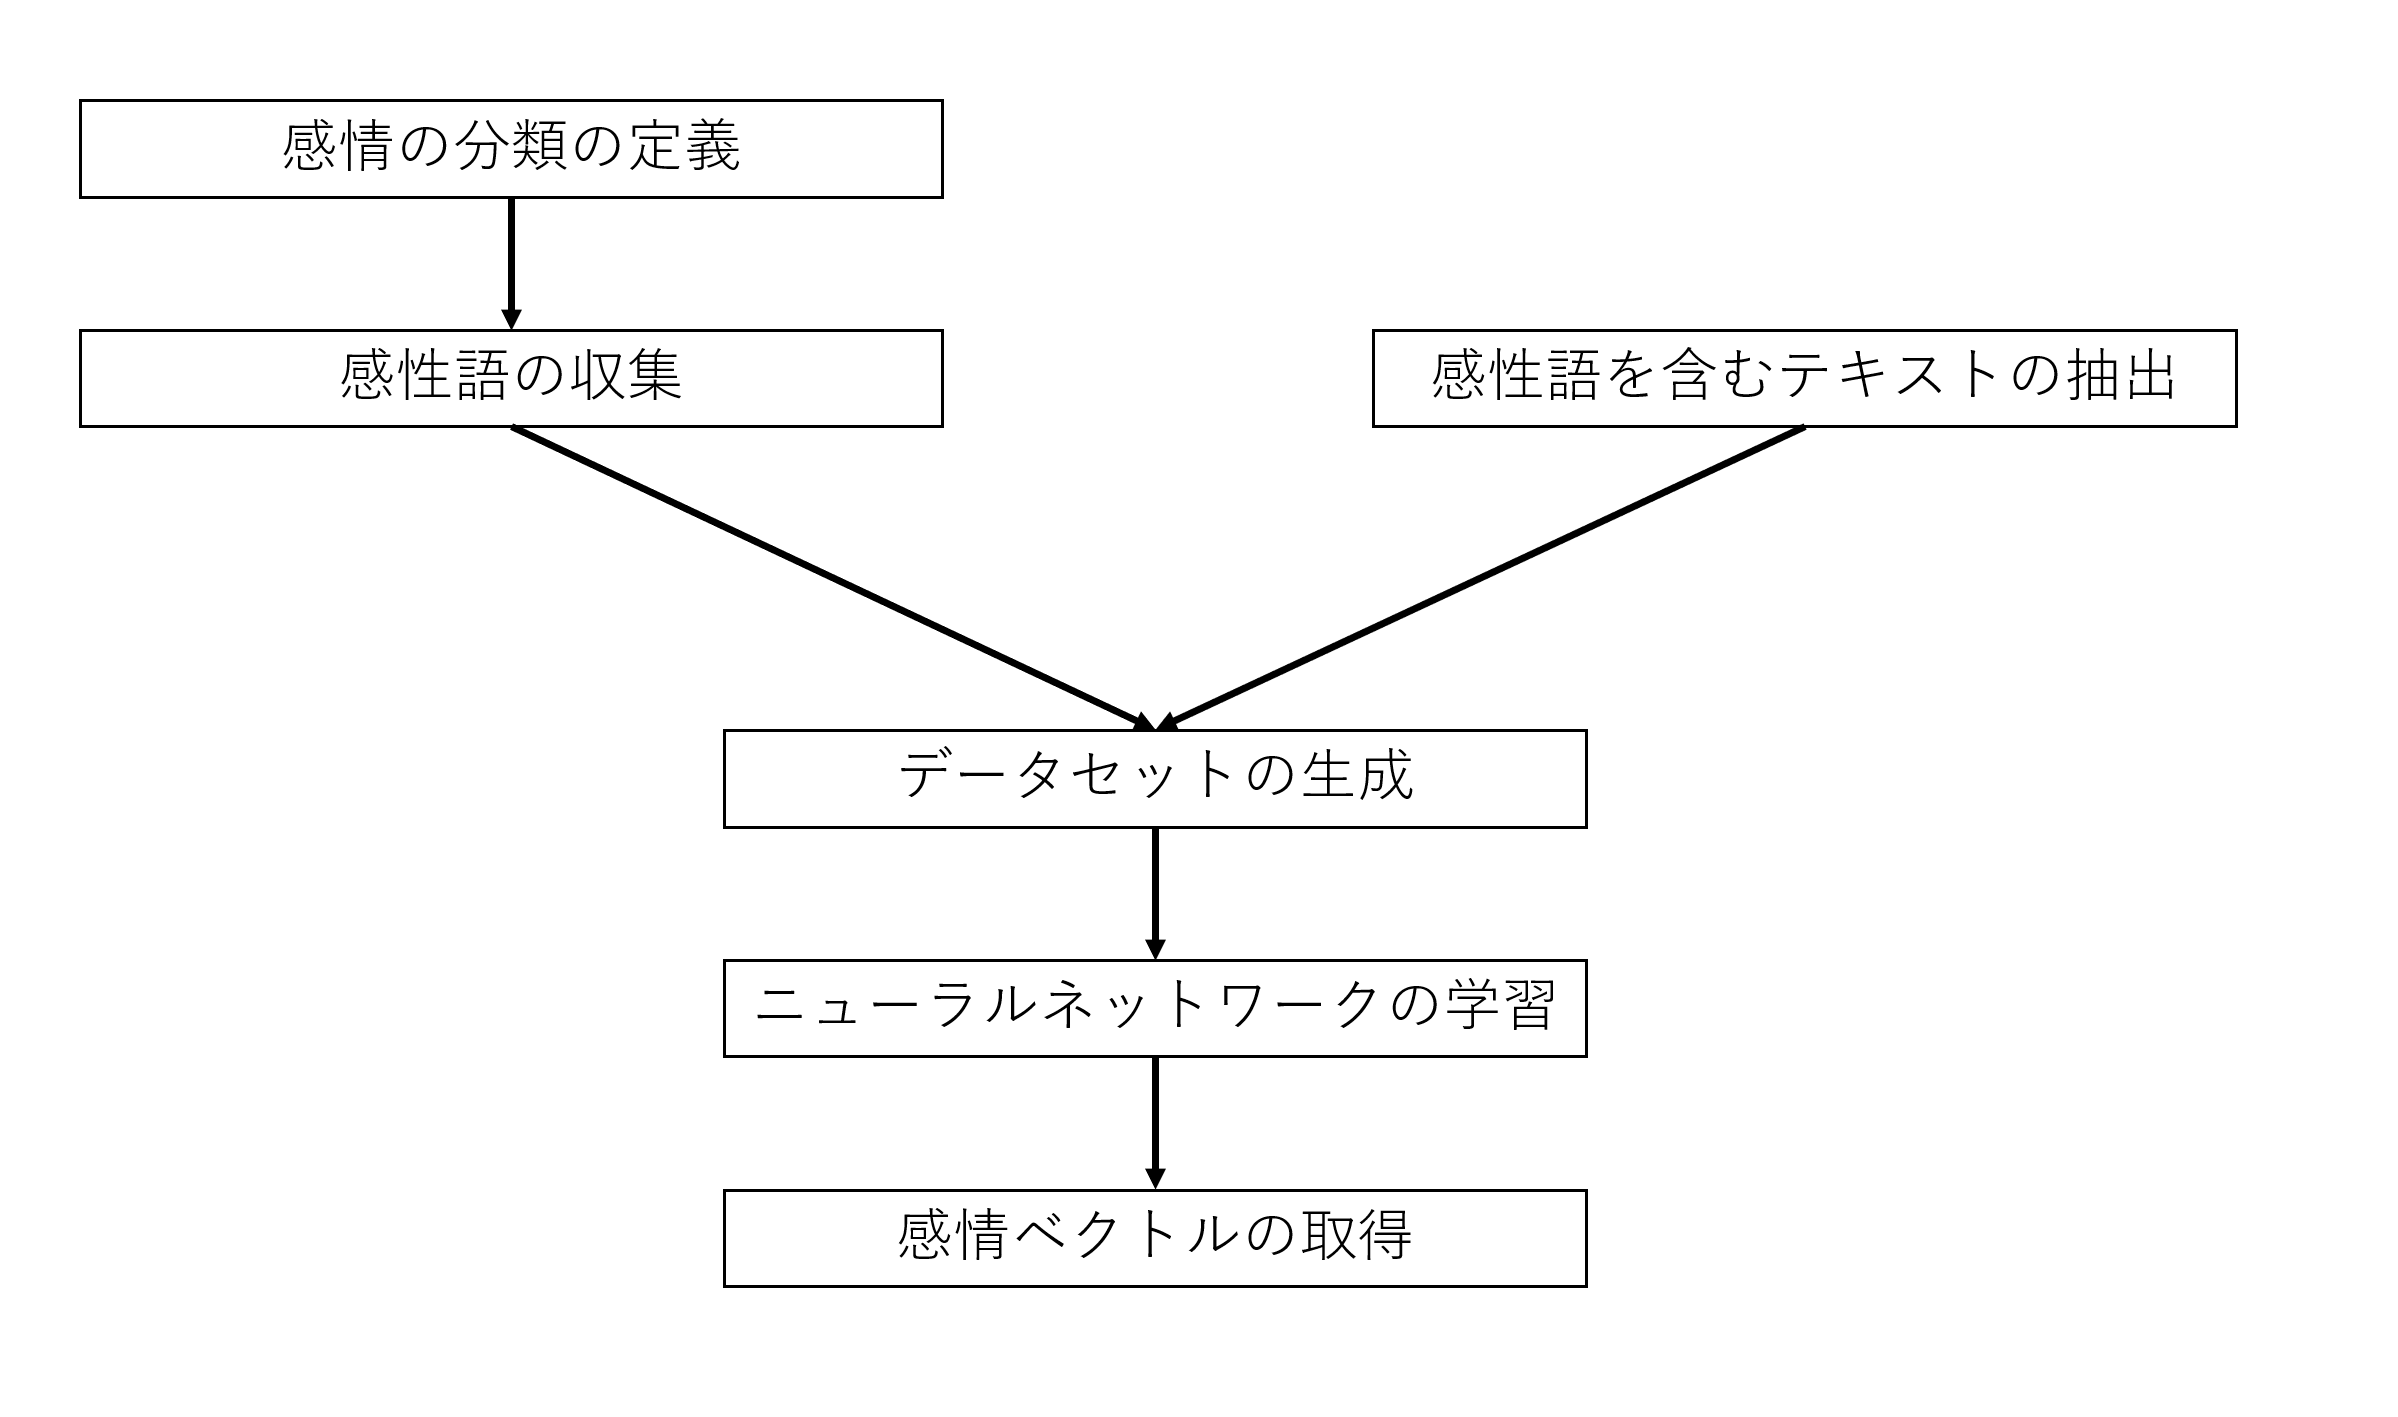
\includegraphics[width=\linewidth]{./figure/flowchart.png}
		\caption{提案手法の流れ}
		\label{fig:flowchart}
	\end{figure}
	分散表現と感情ベクトルを対応付けるに当たり,
	感情表現辞典\cite{kanjou_hyogen_jiten}から取得できる単語である感性語と
	その感情情報を利用する.
	Word2Vecの学習を行う上でもとになっている分布仮説の考え方を応用し,
	感性語の感情が周囲の単語に影響を与えるという仮説のもとでデータセットを生成した.
	分散表現から感情ベクトルへの変換には非常にシンプルなニューラルネットワークを用い,
	学習を行った.
	本手法で作成したシステムでは,文章を入力することによりそれを構成している単語の感情ベクトルを
	入力文の文脈を考慮した上で出力することができる.
	また,入力がBERTの分散表現としたことで,感情ベクトルを出力可能な単語数は
	BERTが扱うことのできる語彙数と一致し,従来の辞書構築型アプローチと比べると
	対応可能語彙数は大幅に増加している.
	以下,本手法の流れについて述べる.



	\section{提案手法の流れ}
		図\ref{fig:whole_image}は,入力されたテキストからそれを構成する各単語の感情情報を抽出するまでの
		全体的な処理の様子を示したものである.
		以下,これに沿って提案手法を説明する.

		\begin{figure}[H]
			\centering
			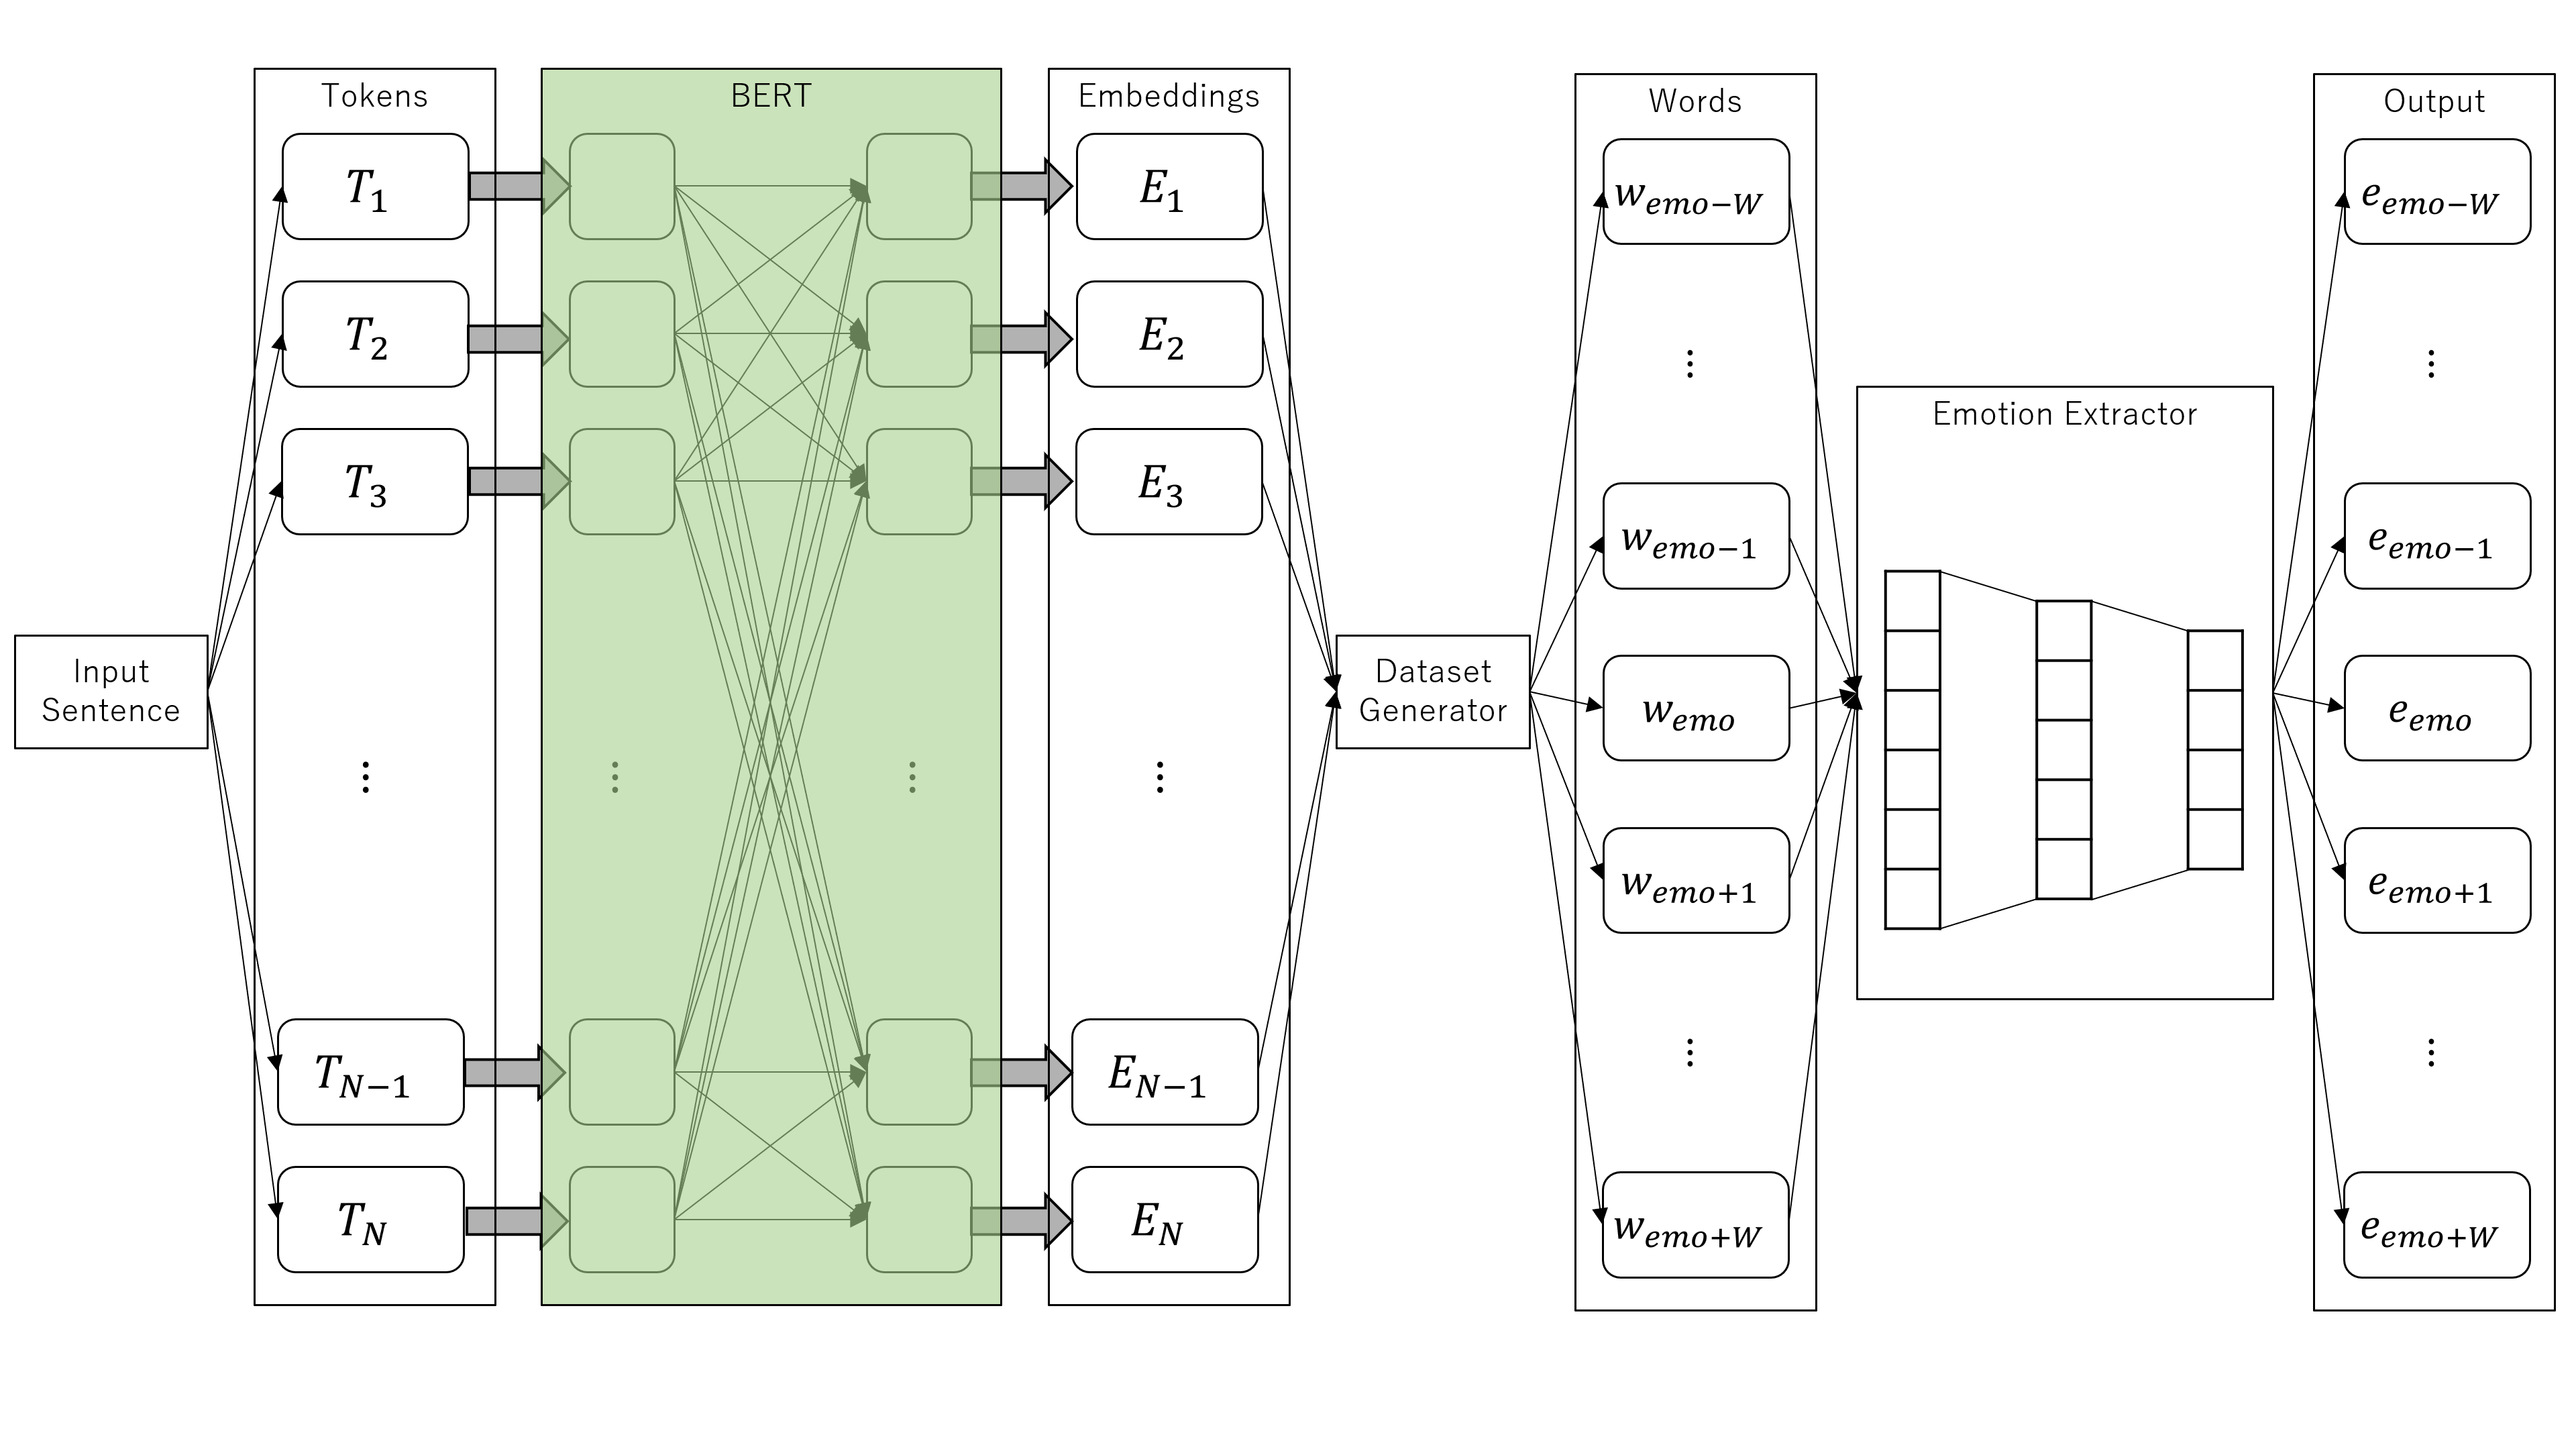
\includegraphics[width=\linewidth]{./figure/whole_image.png}
			\caption{感情情報の抽出における処理の様子}
			\label{fig:whole_image}
		\end{figure}

		\subsection{感情の分類方法の決定}
			本手法における感情分類の方法として,感情表現辞典\cite{kanjou_hyogen_jiten}で
			取得できる感情ベクトルに合わせた10次元の感情分類を採用している.
			各感情は「喜,怒,哀,怖,恥,好,厭,昂,安,驚」である.
			これらの感情は,日本語における言語表現の観点から決められたものである.

		\subsection{感性語の収集}
			感情表現辞典には,各感情を表す単語および熟語が2278語収録されている.
			各単語に対し,該当する感情に1,該当しない感情に0を割り振った10次元の感情ベクトルを
			対にしてリスト化した.
			いくつか例を示す.
			\begin{itemize}
				\item 「めでたい」
				\par $$(喜, 怒, 哀, 怖, 恥, 好, 厭, 昂, 安, 驚)=(1, 0, 0, 0, 0, 0, 0, 0, 0, 0)$$
				\item 「恐ろしい」
				\par $$(喜, 怒, 哀, 怖, 恥, 好, 厭, 昂, 安, 驚)=(0, 0, 0, 1, 0, 0, 0, 0, 0, 0)$$
			\end{itemize}

			また,これらの感性語の中に多数の感情に1が割り振られた単語(以下,感性多義語とよぶ)が存在する.
			感性多義語の例を以下に示す.
			\begin{itemize}
				\item 「気持ち」
				\par $$(喜, 怒, 哀, 怖, 恥, 好, 厭, 昂, 安, 驚)=(1, 1, 0, 0, 0, 0, 1, 0, 1, 0)$$
				\item 「涙」
				\par $$(喜, 怒, 哀, 怖, 恥, 好, 厭, 昂, 安, 驚)=(1, 0, 1, 0, 0, 0, 1, 1, 0, 0)$$
				\item 「思い」
				\par $$(喜, 怒, 哀, 怖, 恥, 好, 厭, 昂, 安, 驚)=(0, 0, 1, 0, 0, 1, 1, 0, 0, 1)$$
			\end{itemize}

			感性多義語には,多数の感情と結びつくような感情ベクトルが与えられるが,
			あらゆる文脈でこれら全ての感情を想起するようなケースは考えにくい.
			つまり,感性多義語については,感情表現辞典で与えられたベクトルをそのまま出力するだけでなく,
			文脈に応じて適切な感情の出力を強調し,不適切な感情の出力を抑えることが求められる.
			
			なお,感情表現辞典に掲載された単語および熟語のうち,
			分かち書きで2単語以上に分かれてしまうものについては
			リストから除外を行った.
			これは,分かち書きで分解された各要素のうち,どの部分に感情情報があるのかを
			判断するのが難しいためである.
			この際,分かち書きには,形態素解析エンジンのMeCab\cite{mecab}を用いた.
			\begin{table}[H]
				\caption{感情表現辞典から取得した感性語の例}
				\label{table:kansei_words}
				\centering
					\begin{tabular}{cc}
						\hline
						感情 & 感性語の例 \\
						\hline \hline
						喜 & めでたい,歓喜,感謝,誇り,$\cdots$ \\
						怒 & 腹立たしい,激怒,憤り,反感,$\cdots$ \\
						哀 & 悲哀,哀悼,嘆き,泣き別れ,$\cdots$ \\
						怖 & 不気味,恐ろしい,震えあがる,戦慄,$\cdots$ \\
						恥 & 照れる,生き恥,羞恥心,赤面,$\cdots$ \\
						好 & 人情,愛する,憧れる,お気に入り,$\cdots$ \\
						厭 & 不快,嫌い,憎しみ,残念,$\cdots$ \\
						昂 & 焦る,緊迫,ときめく,激情,$\cdots$ \\
						安 & 安心,和やか,落ち着く,悠長,$\cdots$ \\
						驚 & たまげる,驚愕,呆然,以外,$\cdots$ \\
						\hline
					\end{tabular}
				\end{table}

		\subsection{感性語を含むテキストデータの取得}
			学習用データセットを作成するにあたり,大量のテキストデータを必要とする.
			しかし,このテキストデータセット自体には感情にかかわるラベル付けがなされている必要はない.
			まず,テキストデータセットを1文ずつに分解したうえで,MeCabによる分かち書きを行い,
			文を構成する各単語の原型のリストを生成した.
			このリスト内に感性語が含まれているような文だけを抜粋し,
			図\ref{fig:whole_image}における"Input Sentece"に対応する
			学習用データセット作成のための入力文とした.

		\subsection{データセットの生成}
			感性語を含むテキストをBERTに入力するにあたり,BERTのトークナイザで入力文をトークン化する.
			これは図\ref{fig:whole_image}の"Input Sentence"から"Tokens"への変換に対応する.
			BERTのトークナイザはMeCabによる形態素解析とwordpieceアルゴリズムによるサブワード分割により構成されている.
			トークン化されたテキストをBERTに入力すると,図\ref{fig:whole_image}の"Embeddings"に対応する,
			各トークンの分散表現を取得することができる.

			以下,図\ref{fig:whole_image}の"Dataset Generator"に対応する処理について述べる.
			まず,感性語の周辺単語の収集を行う.
			ウィンドウサイズを$W$としたとき,感性語の前後それぞれ$W$個の単語を収集する.
			なお,サブワード分割されたトークンは結合した状態でウィンドウサイズをカウントする.
			その際には,名詞,形容詞,形容動詞,動詞以外はカウント対象外とした.
			また,名詞のうち,代名詞,接尾語,非自立語,数詞についても除外を行った.
			これらの単語が感情情報を持つとは考えにくいためである.

			感性語が持っている感情ベクトルを図\ref{fig:whole_image}の"Words"に対応する,
			ウィンドウサイズ内の単語すべてに付与することにより,
			学習用データセットは生成されることになる.
			つまり,ウィンドウサイズ内のトークンに対応する分散表現と感情ベクトルのペアが1件のデータ
			ということになる.
			以下に例を示す.

			図\ref{fig:token_processing}は,
			入力テキストとして「道の真ん中で転んでしまい恥ずかしかったので,走ってその場を立ち去った」
			という文章を与えたときのトークン処理の様子である.
			この文章をBERTへ入力するために,まずトークン化を行う.
			ここで,"\#\#"で始まるトークンが存在するが,これは分かち書きの後さらに
			サブワード分割がなされたために生じるトークンである.
			よって,品詞による判別を行うためにはサブワード分割されたトークンを結合する必要性がある.
			サブワード結合状態での分割単位で品詞を調査し,
			ウィンドウサイズのカウント対象となるトークン列を絞り込む.
			\begin{figure}[H]
				\centering
				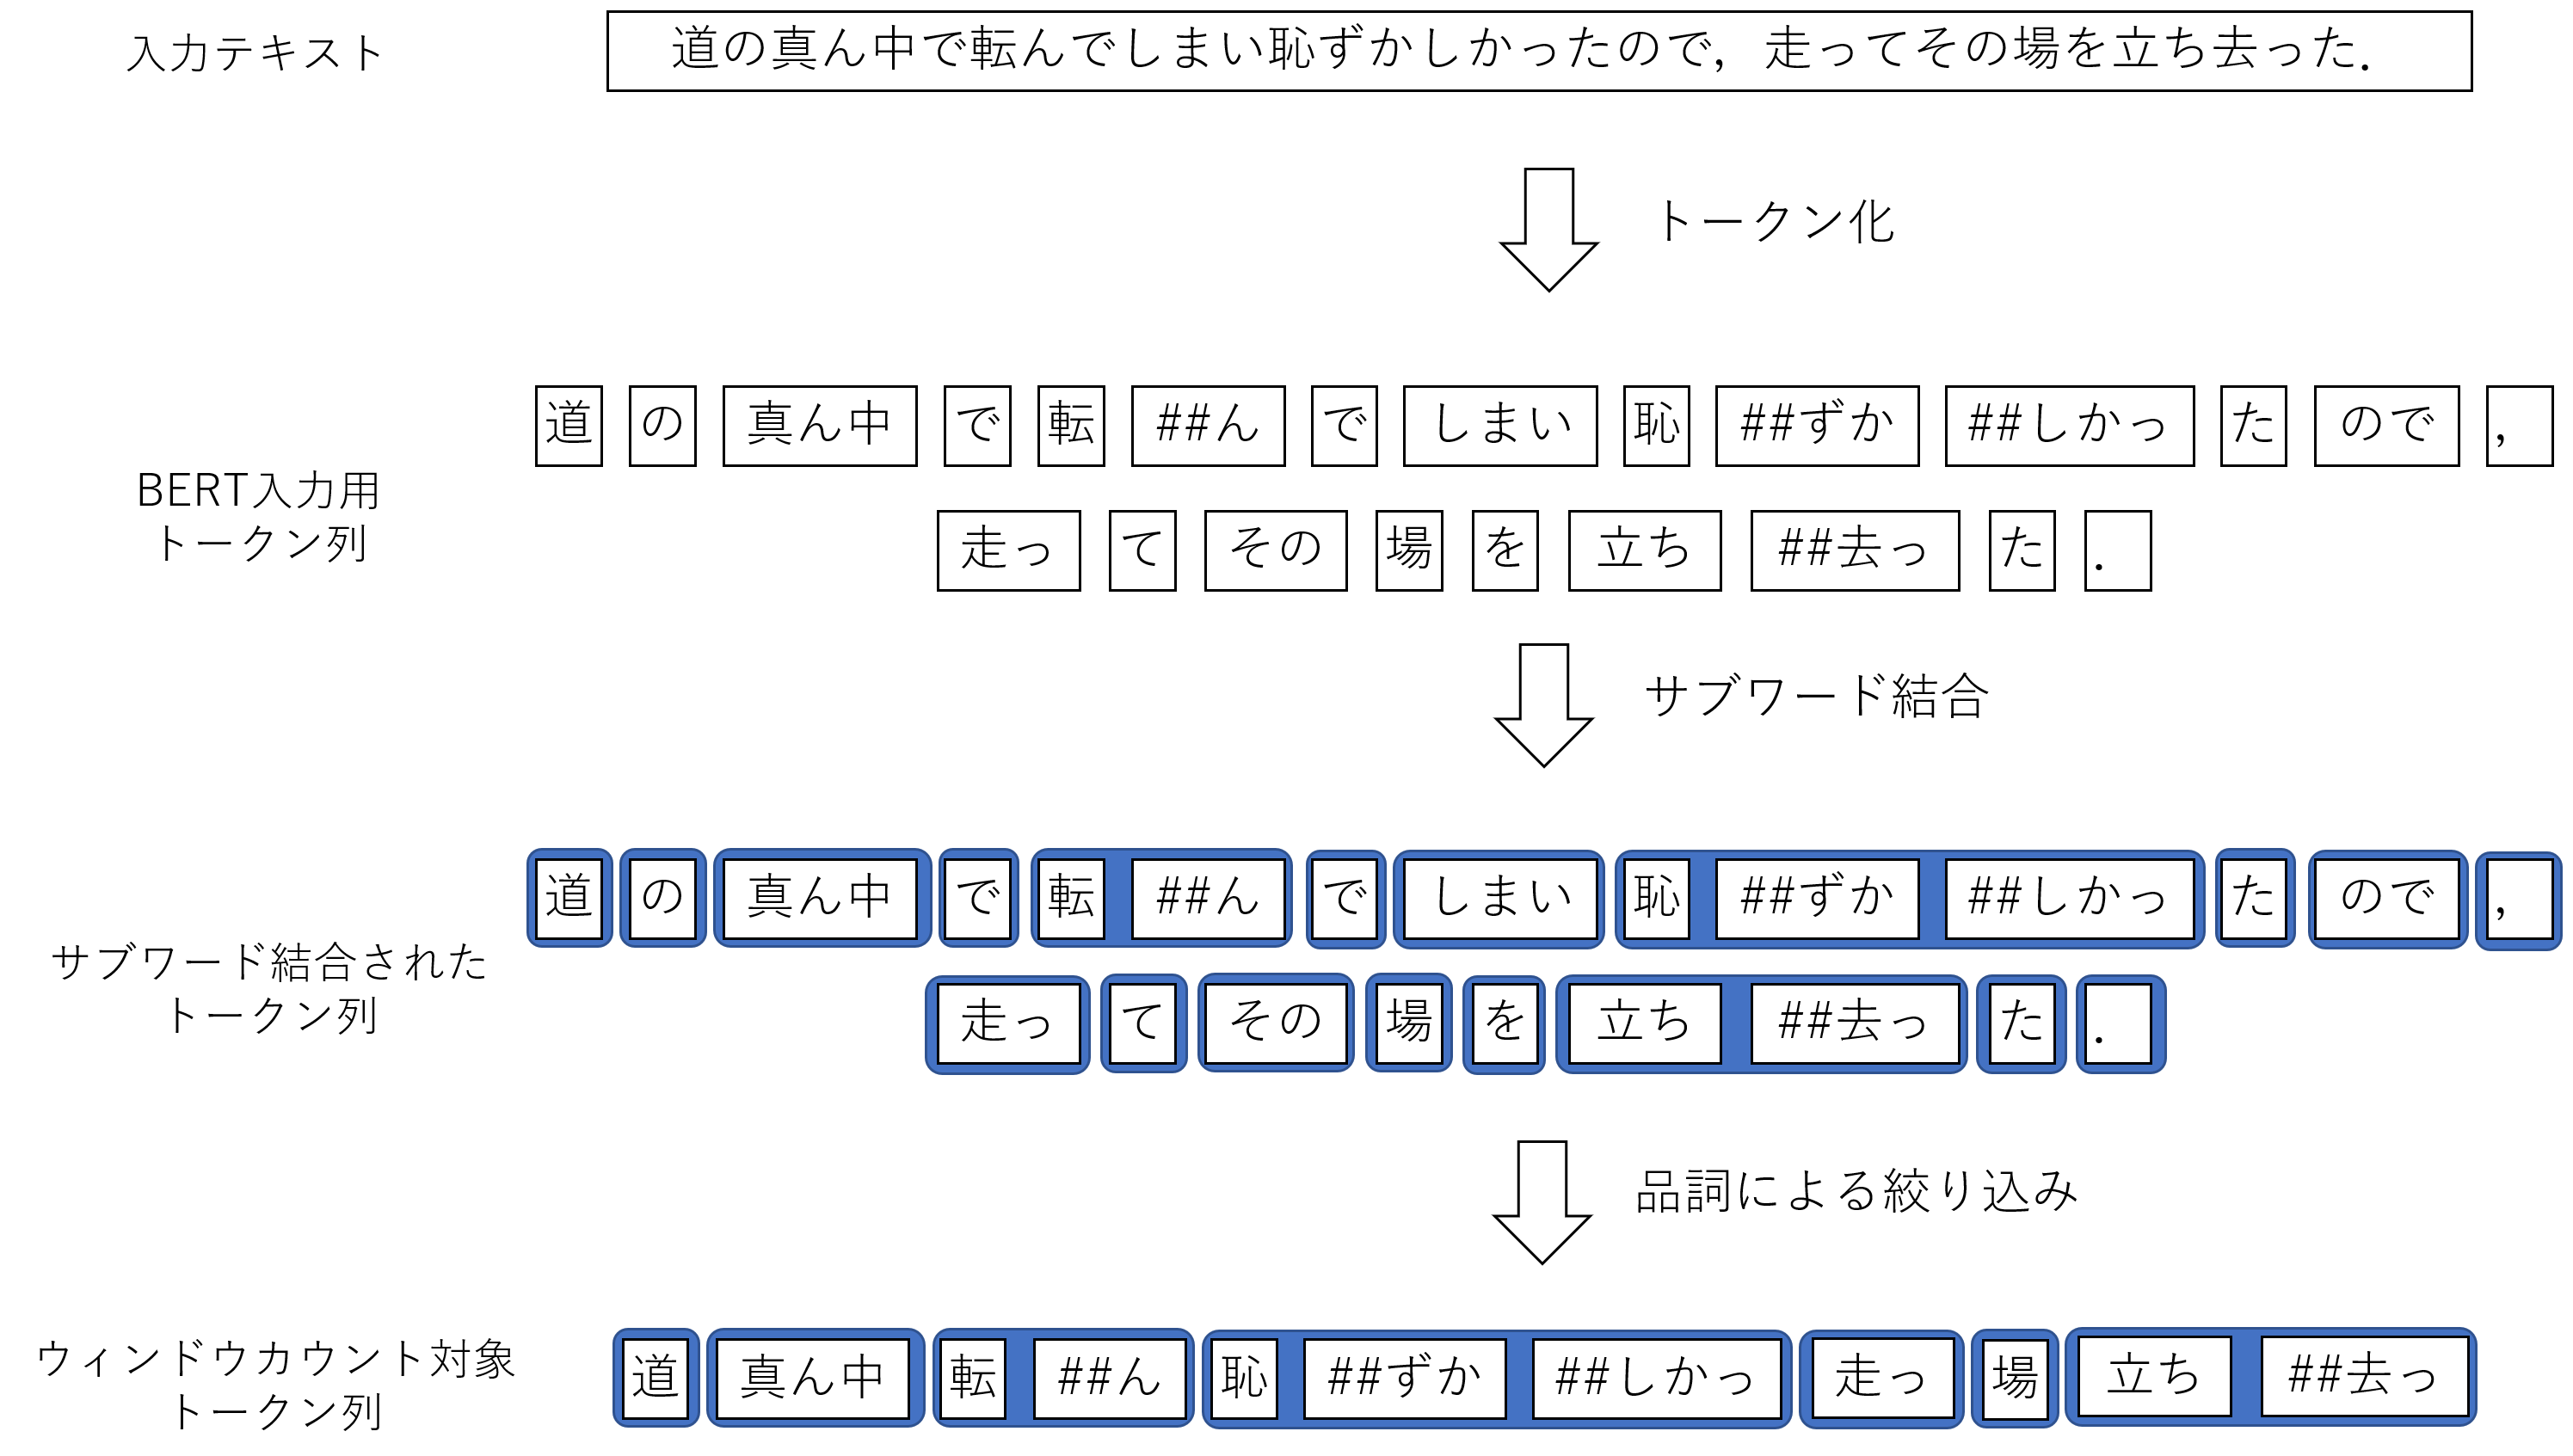
\includegraphics[width=\linewidth]{./figure/token_processing.png}
				\caption{入力文から生成されるトークンの処理の様子}
				\label{fig:token_processing}
			\end{figure}
			これらのトークン列のうち,「恥 \#\#ずか \#\#しかっ」の原型である「恥ずかしい」が
			感性語となる.
			よって,以下のような感情ベクトルを感情表現辞典から取得することができる.
			$$(喜, 怒, 哀, 怖, 恥, 好, 厭, 昂, 安, 驚)=(0, 0, 0, 0, 1, 0, 0, 0, 0, 0)$$
			ウィンドウサイズを3としたとき,「恥 \#\#ずか \#\#しかっ」の前後それぞれ3つずつの
			トークン列へ同様の感情ベクトルを付与することになる.
			図\ref{fig:make_dataset_window}は,この様子を図式化したものである.
			\begin{figure}[H]
				\centering
				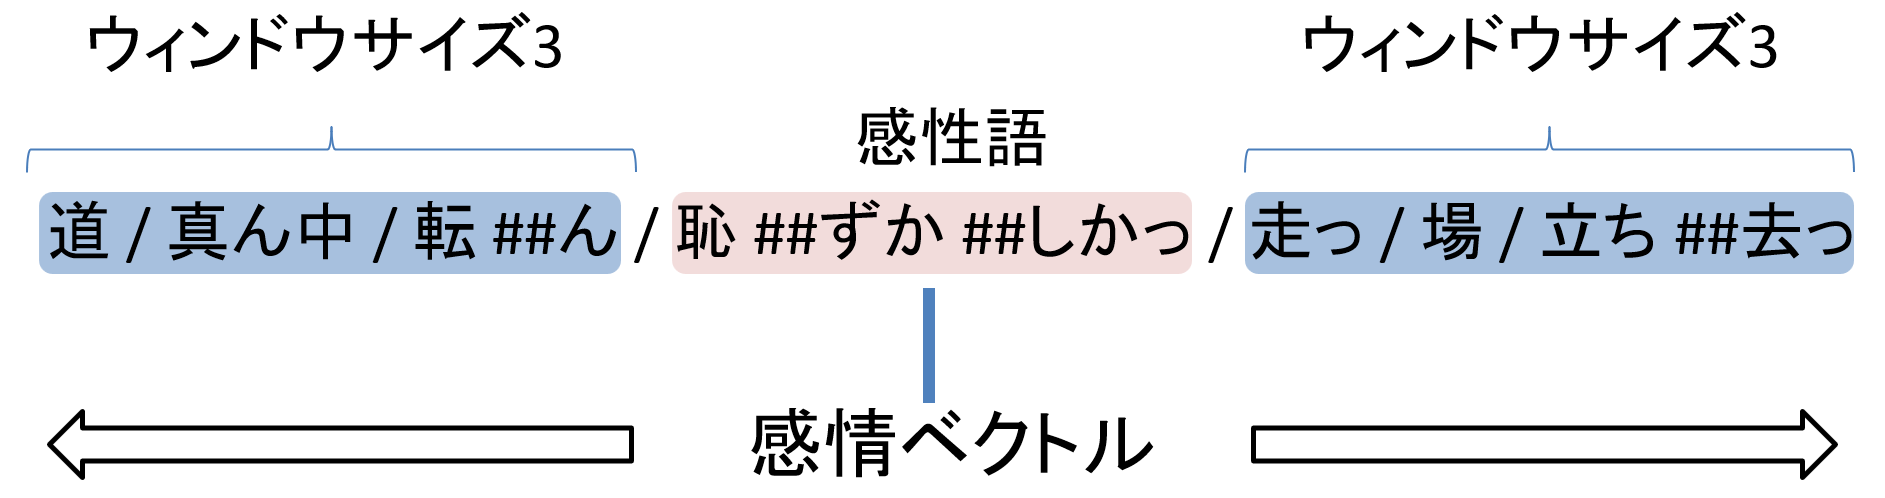
\includegraphics[width=\linewidth]{./figure/dataset_make_window.png}
				\caption{中心の感性語が持つ感情ベクトルを周辺単語へ付与する様子}
				\label{fig:make_dataset_window}
			\end{figure}


			また本手法ではデータセット生成に当たり,
			与える感情ベクトルについて感性語と周辺単語の距離に応じた重み付けを行った。
			感性語との距離が離れるほど、与えられる感情ベクトルの強度が弱くなる。
			これは,感性語ではない一般単語が感性語と同等の強度でその感情を想起するわけではない,
			という仮説に基づくものである.
			表\ref{table:vector_weaken}は最小値を0.5とした上で感性語との距離に応じて
			等間隔に値が小さくなるよう感情ベクトルを付与している様子を表している.
			\begin{table}[H]
				\centering
				\caption{感性語からの距離に応じて感情ベクトルの強度を弱める様子}
				\label{table:vector_weaken}
					\begin{tabular}{cccccccccc}
						\hline
						感性語との距離 & -4 & -3 & -2 & -1 & 0 & +1 & +2 & +3 & +4 \\
						\hline
						ベクトル強度 & 0.5 & 0.625 & 0.75 & 0.875 & 1.0 & 0.875 & 0.75 & 0.625 & 0.5 \\
						\hline
					\end{tabular}
			\end{table}

		\subsection{ニューラルネットワークの学習}
			本手法では,BERTが出力するトークンの分散表現から感情ベクトルを出力するために,
			非常にシンプルなニューラルネットワークを採用し,学習を行った.
			これは図\ref{fig:whole_image}の"Emotion Extractor"に対応する.
			以下の図\ref{fig:network}は、用いるネットワークを図式化したものである。
			\begin{figure}[H]
				\centering
				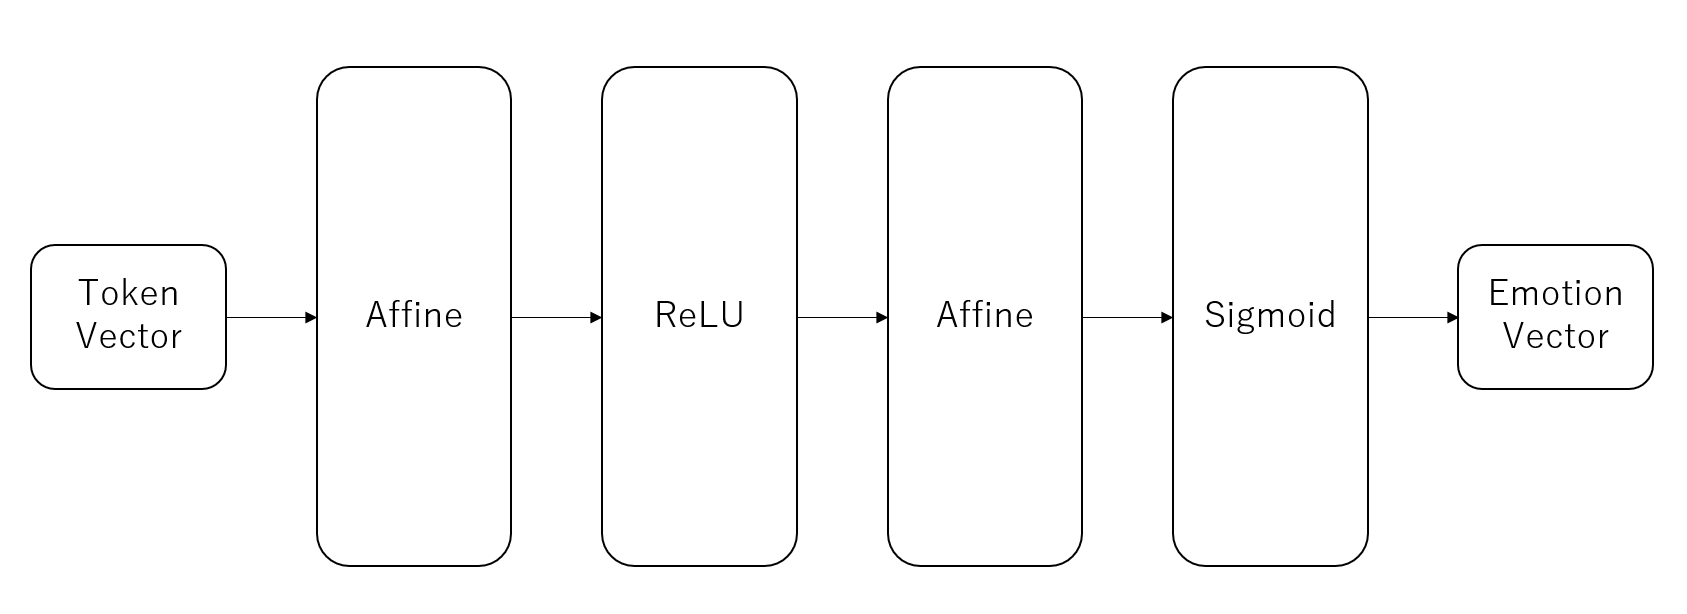
\includegraphics[width=\linewidth]{./figure/network.png}
				\caption{ニューラルネットワークの構造}
				\label{fig:network}
			\end{figure}
			具体的には,入力層が768次元の分散表現,出力層が10次元の感情ベクトルとなるため,
			400次元の中間層を設けた3層のニューラルネットワークを学習させた.
			中間層の活性化関数はReLU関数\cite{relu}とし,
			出力層にはSigmoid関数をかけ、0から1の値へ変換を施している。
			ReLU関数,Sigmoid関数はそれぞれ以下の式で示される.
			\begin{equation}
				ReLU(x)=
				\left\{
				\begin{alignedat}{2}
					x\;\;\;(x>0) \\
					0\;\;\;(x\leqq0)
				\end{alignedat}
				\right.
			\end{equation}
			\begin{equation}
				Sigmoid(x)=\frac{1}{1+e^{-x}}
			\end{equation}

			この時出力された10次元のベクトルが,
			データセットに与えられた感情ベクトルに近づくよう学習を行う.
			損失関数は最小二乗誤差とした.

		\subsection{感情ベクトルの取得}
			以上のようにして学習したネットワークに,BERTから得られたトークンの分散表現を入力することにより,
			入力文全体の文脈を踏まえた感情ベクトルを出力することができる.
			出力対象単語は,データセット作成時のウィンドウサイズカウント対象になる単語と
			同等の条件を満たすものに絞っている.
			また,サブワードに別れてしまう単語については,
			それぞれのトークンに対して出力される感情ベクトルの平均値をまとめて出力する.

			本手法では,出力に正規化を行わなかった.
			その理由としては,感情表現辞典から得られる感情ベクトルには
			複数の感情のラベルがついた単語が存在していること,
			1感情に対してだけわずかに値が出力されるようなケースでは
			その値が極端に大きくなってしまう可能性があることが挙げられる.
